\vspace{-2em}

\begin{figure}[H]
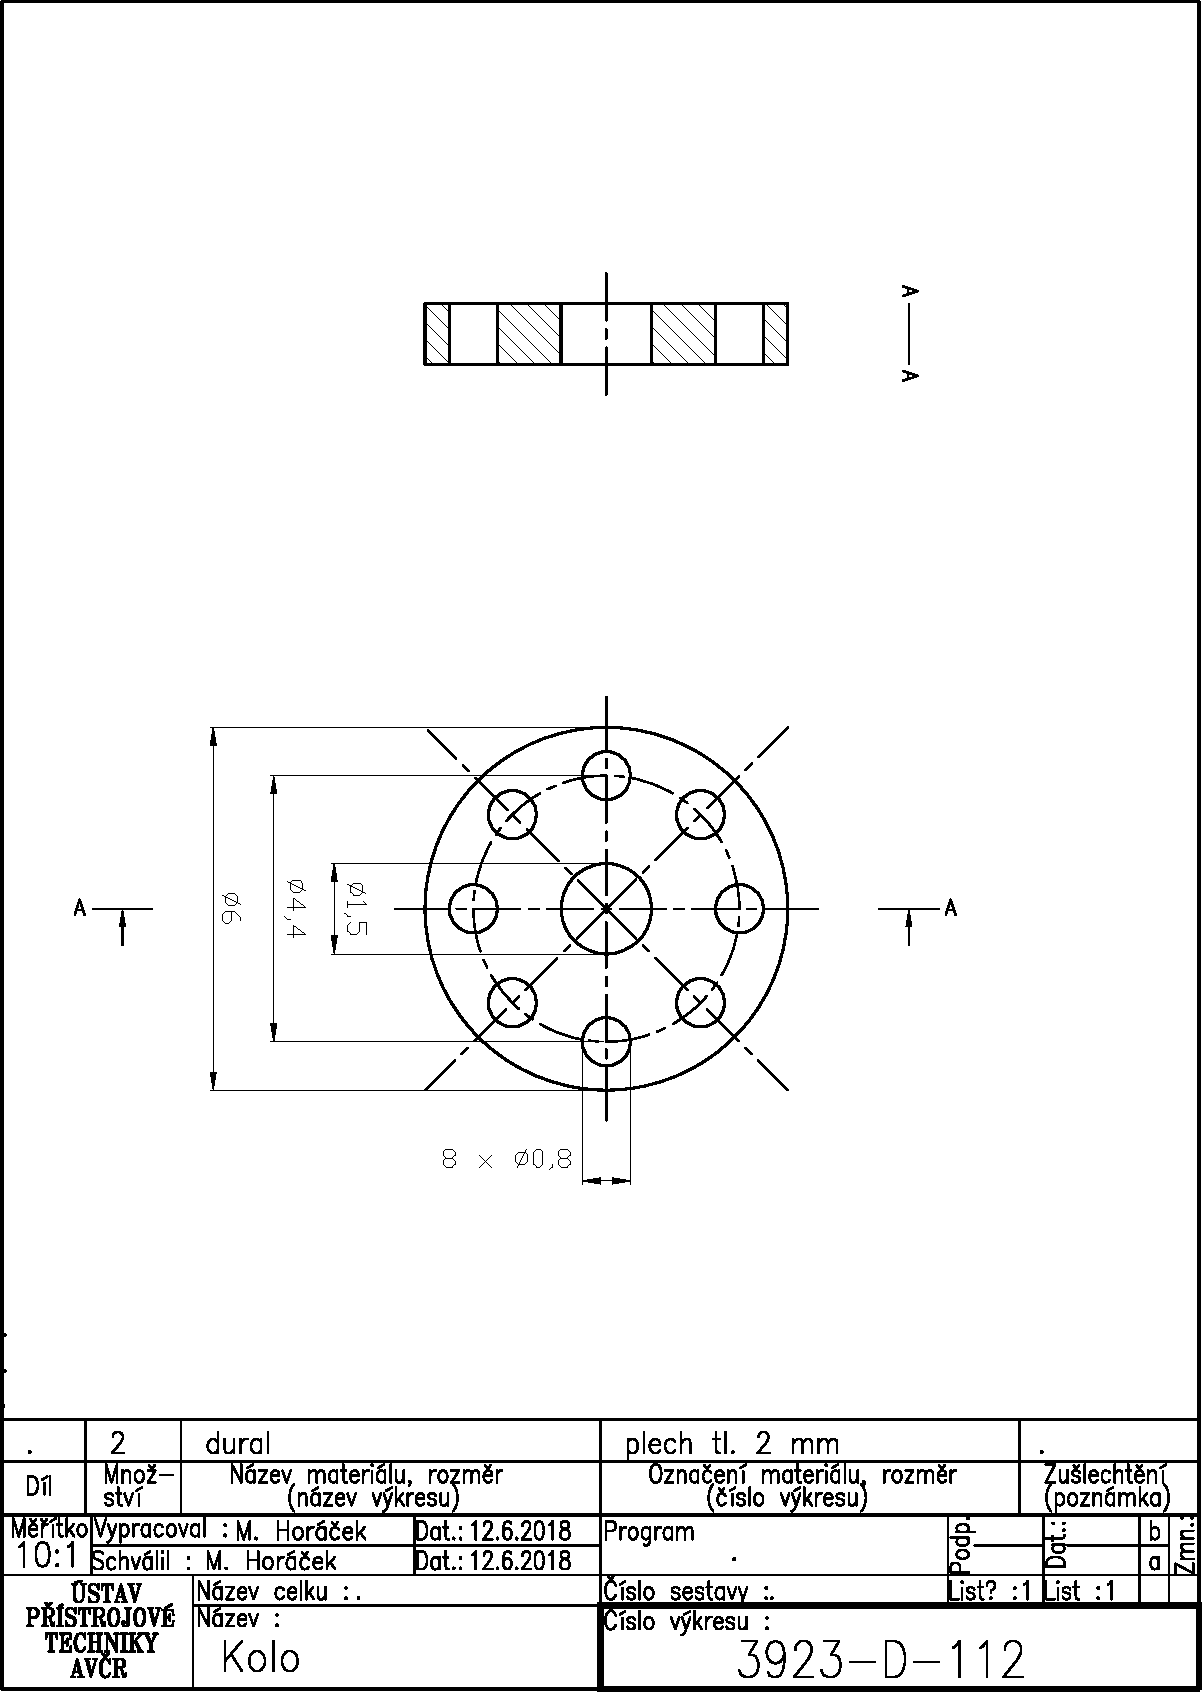
\includegraphics[width=0.95\textwidth]{data/wheel.pdf}
\caption{Výkres perforovaného kola. Autor: Miroslav Horáček.}
\label{fig:final-wheel}
\end{figure}

\begin{figure}[h]
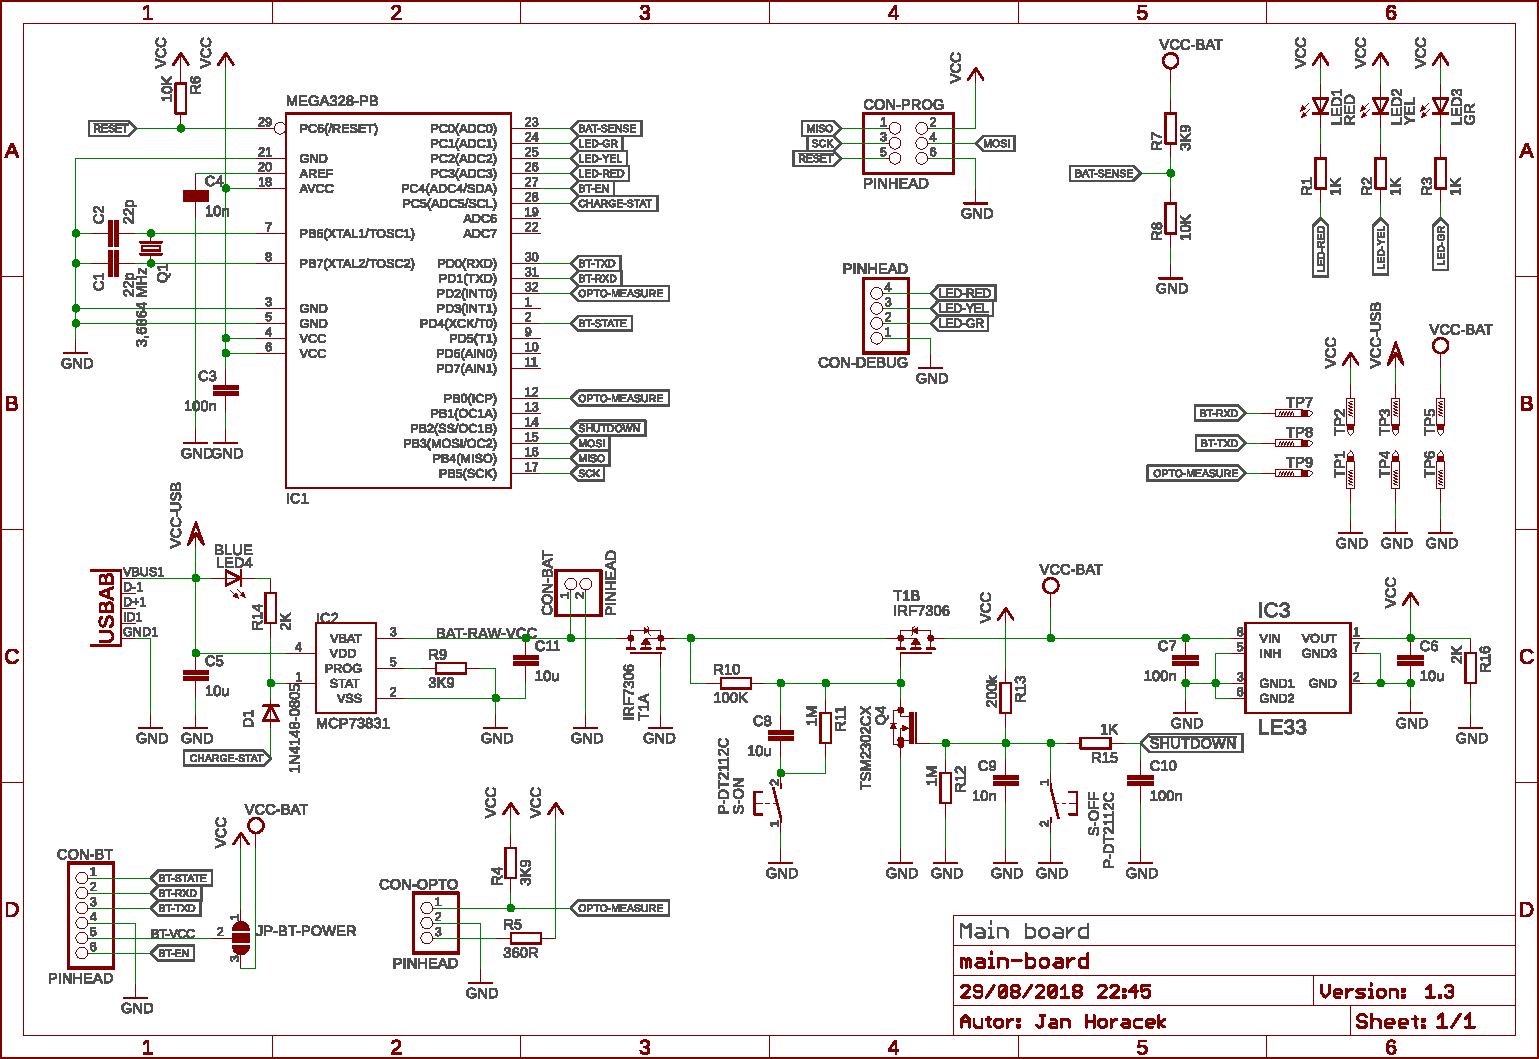
\includegraphics[angle=90,width=\textwidth]{data/wsm_main_board_v1_3.pdf}
\caption{Schéma hlavní DPS měřicího vozu.}
\label{fig:wsm-sch}
\end{figure}

\begin{table}[h]
	\begin{tabularx}{0.66\textwidth}{rrX}
		\toprule
		Jízdní stupeň & Rychlost [modelový km/h] \\
		\midrule
		1 & 1 \\
		2 & 2 \\
		3 & 4 \\
		4 & 6 \\
		5 & 8 \\
		\textbf{6} & \textbf{10} \\
		7 & 12 \\
		8 & 15 \\
		9 & 17 \\
		\textbf{10} & \textbf{20} \\
		11 & 22 \\
		12 & 25 \\
		\textbf{13} & \textbf{30} \\
		14 & 35 \\
		\textbf{15} & \textbf{40} \\
		16 & 45 \\
		\textbf{17} & \textbf{50} \\
		18 & 55 \\
		\textbf{19} & \textbf{60} \\
		20 & 65 \\
		\textbf{21} & \textbf{70} \\
		22 & 75 \\
		\textbf{23} & \textbf{80} \\
		24 & 85 \\
		\textbf{25} & \textbf{90} \\
		\textbf{26} & \textbf{100} \\
		\textbf{27} & \textbf{110} \\
		\textbf{28} & \textbf{120} \\
		\bottomrule
	\end{tabularx}
	\caption{Rychlostní tabulka dle standardu KMŽ Brno~I, vybrané kalibrované
	kroky jsou vyznačeny tučne, zbytek je interpolován.}
	\label{fig:step-to-speed}
\end{table}
